\label{subsec:formulation}
Let $X = \{ \mathbf{x}^1, \ldots, \mathbf{x}^n \}$ be a variable that represents the $n$ locations of 
a set of fiducials.
Let $\hat{X}$ denote the true locations of fiducial features in any given image $I$, while $X_k$ refer
to ground truth fiducials in the exemplar set used in our algorithm, where $k = 1 \ldots K $ indexes
into the set of exemplars in consideration. In this paper, we consider $K = 20, \; \& \; n = 20$
since that is the set of common fiducials detected by algorithms presented in recent
literature~\cite{xhuCVPR12_wild,xiongCVPR13_SDM,artizzzuICCV13_COFW,asthanaCVPR14_Chehra,Tzimiropoulos_2015_CVPR}. Note that
recent approaches~\cite{smithECCV14_ED} offer a way to increase the number of common fiducial
locations, and thus our assumption is not restrictive.
Let $R = \{ \mathbf{r}^1, \ldots, \mathbf{r}^m \}$ represent features extracted at $m$ pixels on the
image. We would like to optimize the following function to obtain the fiducial locations at the
current image 
\begin{equation}
  X^* = \arg\max_{\tilde{X}} P( X~|~R )
  \label{eq:main_equation}
\end{equation}
Note that $\tilde{X}$ is the space of all possible sets of fiducial locations. It is a huge
($40$ dimensional) space, and sampling all of it is impractical. Instead, let us assume that we have
been given some candidate locations where probability of a correct result is higher, and assume we
will pick $X$ from one of these locations. Let us depict
these locations with the variable $\mathcal{X} = \{\bar{X}_1, \ldots, \bar{X}_l \}$, where $\bar{X}_i,
i = 1\ldots l$ are the number of candidates we have selected. We can now re-write equation~\ref{eq:main_equation} as
\begin{eqnarray}
  X^* = \arg\max_{\tilde{X}} P( X~|~R, \mathcal{X} )  = \arg\max_i P(\bar{X}_i | R ) 
  \label{eq:main_second_equation}
\end{eqnarray}
where we assume that the probability of selecting fiducials not represented by candidate algorithms
is negligible. Using Bayes rule, and adopting a similar strategy of marginalizing over exemplars used
in~\cite{kumarPAMI13_faceExem}, equation~\ref{eq:main_second_equation} can now be
elaborated as
\begin{eqnarray}
  P( \bar{X}_i~|~R ) & \propto & P( R~|~\bar{X}_i ) \\
  & \propto & \sum_{k\in K} P( R~|~X_k, \bar{X}_i) P( X_k~|~\bar{X}_i )
  \label{eq:main_third_equation}
\end{eqnarray}
where we marginalize over all exemplars $X_k$. Note that
equation~\ref{eq:main_third_equation} \emph{splits} the probability into comparison between
\emph{appearances} of our candidates and exemplars (first term), and comparison between their
shapes (term 2). Further, given structure is preserved in the way these two sets of candidates are 
generated, we can breakdown the above equation into parts
\begin{equation}
  P( \bar{X}_i~|~R ) \propto \sum_{k\in K} \prod_j P( R~|~\mathbf{x}_k^j, \bar{\mathbf{x}}_i^j) P( \mathbf{x}_k^j~|~\bar{\mathbf{x}}_i^j )
  \label{eq:main_fourth_equation}
\end{equation}
We denote individual probabilities for shape and appearance using the following functions
\begin{eqnarray}
  P( R~|~\mathbf{x}_k^j, \bar{\mathbf{x}}_i^j) & = & (1/\alpha) \exp( -\Vert F_k^j - F_i^j \Vert^2 ) 
  \label{eq:app_equation} \\
  P( \mathbf{x}_k^j~|~\bar{\mathbf{x}}_i^j )  & = & (1/\beta) \; dist( \mathbf{x}_k^j, \bar{\mathbf{x}}_i^j )
  \label{eq:shape_equation}
\end{eqnarray}
where $F$ denotes concatenation SIFT and HOG features, while $dist$ is a scaled inverse Euclidean
distance function and $\alpha$, $\beta$ are normalization constants to ensure both equations represent valid probabilities. Note that evaluating equation~\ref{eq:main_fourth_equation} 
entails summing over SIFT and HOG distances between candidate and exemplar fiducials.
Finally, one could alternatively choose to optimize equation~\ref{eq:main_second_equation} using
an optimization function as outlined in section~\ref{subsec:optimization}.
In this work, candidates are generated using algorithms of Zhu \etal~\cite{xhuCVPR12_wild}, 
Xiong \etal~\cite{xiongCVPR13_SDM}, Asthana \etal~\cite{asthanaCVPR14_Chehra}, Artizzu
\etal~\cite{artizzzuICCV13_COFW}, and Tzimiropouluos \etal~\cite{Tzimiropoulos_2015_CVPR}.

\subsection{Example}
In equation~\ref{eq:main_fourth_equation}, the term $P( R~|~\mathbf{x}_k^j,\bar{\mathbf{x}}_i^j )$
can be seen as the term that \emph{selects} appropriate exemplars given fiducial candidates 
using a \emph{shape/appearance constraint} represented by equation~\ref{eq:app_equation}. This is better
illustrated with an example. In Figure~\ref{fig:example_illustration}, we show an input image
for which the \emph{minimum distance} in SIFT+HOG space from a set of exemplars is shown in 
Figure~\ref{fig:distance_map}, for a single fiducial (eye corner). Note how there are several
minima in the distance map (marked by bounding boxes). Running candidate detection algorithms,
however, generates eye fiducial candidates only in a specific region (Figure~\ref{fig:fid_locations}, with
bounding box), which is then selected and isolated using equation~\ref{eq:shape_equation}
(Figure~\ref{fig:distance_constrained}), leading to a correct location of the eye fiducial in the
final output (Figure~\ref{fig:final_output}).

\begin{figure*}
  \centering
  \subfloat[Input Image]{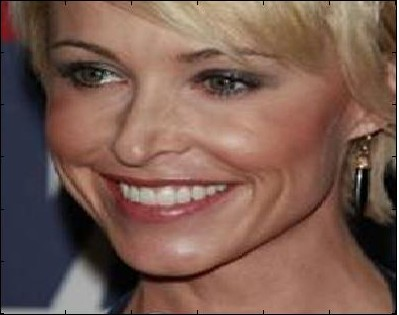
\includegraphics[width=1in,height=0.9in]{fid/figures/im.jpg}}
  \subfloat[Distance from Exemplars]{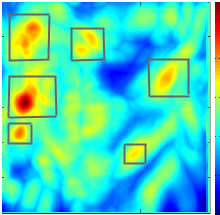
\includegraphics[width=1.5in,height=0.9in]{fid/figures/local_minima_distance.png}\label{fig:distance_map}}
  \subfloat[Output of Fiducials]{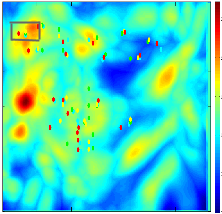
\includegraphics[width=1.5in,height=0.9in]{fid/figures/local_minima_fiducials.png}\label{fig:fid_locations}}
  \subfloat[Constrained Distance]{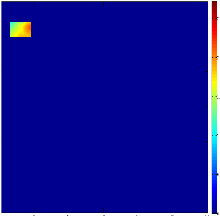
\includegraphics[width=1.5in,height=0.9in]{fid/figures/local_minima_constrained.png}\label{fig:distance_constrained}}
  \subfloat[Final Result]{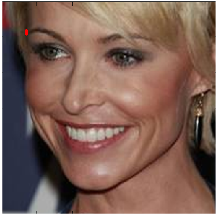
\includegraphics[width=1in,height=0.9in]{fid/figures/local_minima_final_output.png}\label{fig:final_output}}
  \caption{An example of fiducial detection of eye corner in a test image. Best viewed in color.}
  \label{fig:example_illustration}
\end{figure*}
